\documentclass[11pt,a4paper]{report}
\usepackage{amsmath,amsfonts,amssymb,amsthm,epsfig,epstopdf,url,array,graphicx}
\usepackage[english]{babel}


\theoremstyle{plain}
\newtheorem{thm}{Theorem}[section]
\newtheorem{lem}[thm]{Lemma}
\newtheorem{fact}{Fact}[chapter]
\newtheorem{assm}{Assumption}[chapter]
\newtheorem*{assm*}{Assumption}
\newtheorem{prop}[thm]{Proposition}
\newtheorem*{cor}{Corollary}

\theoremstyle{definition}
\newtheorem{defn}{Definition}[chapter]
\newtheorem{conj}{Conjecture}[section]
\newtheorem{exmp}{Example}[section]

\theoremstyle{remark}
\newtheorem*{rem}{Remark}
\newtheorem*{note}{Note}


\title{Notes on Scalable Blockchain Protocols (version 0.0.2)}
\date{March 14-April 12, 2015}
\author{Vitalik Buterin (Ethereum) \\  \\ Reviewers and collaborators: Gavin Wood, Vlad Zamfir (Ethereum), \\ Jeff Coleman (Kryptokit), \\ Eric Lombrozo (Ciphrex)}

\begin{document}

\maketitle

\chapter{Introduction}

Currently, all blockchain consensus protocols that are actively in use have a critical limitation: every node in the network must process every transaction. Although this requirement ensures a very strong guarantee of security, making it all but impossible for an attacker even with control over every node participating in the consensus process to convince the network of the validity of an invalid transaction, it comes at a heavy cost: every blockchain protocol that works in this way is forced to choose between limiting itself to a low maximum transaction throughput, with a resulting high per-transaction cost, and allowing a high degree of centralization.

What might perhaps seem like a natural solution, splitting the relevant data over a thousand blockchains, has the two fundamental problems that it (i) decreases security, to the point where the security of \emph{each individual blockchain} on average does not grow \emph{at all} as total usage \emph{of the ecosystem} increases, and (ii) massively reduces the potential for interoperability. Other approaches, like merge-mining, seem to have stronger security, though in practice such approaches are either very weak in more subtle ways \cite{mmpetertodd} - and indeed, merged mined blockchains have successfully been attacked\cite{coiledcoin} - or simply fail to solve scalability, requiring every consensus participant to process every blockchain and thus every transaction anyway.

There are several reasons why scalable blockchain protocols have proven to be such a difficult problem. First, because we lose the guarantee that a node can personally validate every transaction in a block, nodes now necessarily need to employ statistical and economic means in order to make sure that other blocks are secure; in essence, every node can only \emph{fully} keep track of at most a few parts of the entire "state", and must therefore be a "light client", downloading only a small amount of header data and not performing full verification checks, everywhere else. Second, we need to be concerned not only with validity but also with data availability; it is entirely possible for a block to appear that looks valid, and is valid, but for which the auxiliary data is unavailable, leading to a situation where no other validator can effectively validate transactions or produce new blocks since the necessary data is unavailable to them. Finally, transactions must necessarily be processed by different nodes in parallel, and given that it is not possible to parallelize arbitrary computation \cite{parallelcomputing}, we must determine the set of restrictions to a state transition function that will best balance parallelizability and utility.

This paper proposes another set of strategies for achieving scalability, as well as some formalisms that can be used when discussing and comparing scalable blockchain protocols. Generally, the strategies revolve around a "sample-and-fallback" game: in order for any particular block to be valid, require it to be approved by a randomly selected sample of validators, and in case a bad block does come through employ a mechanism in which a node can challenge invalid blocks, reverting the harmful transactions and transferring the malfeasant validators' security deposit to the challengers as a reward unless the challenge is answered by a confirmation of validity from a much greater number of validators. Theoretically, under a Byzantine-fault-tolerant model of security, fallback is unnecessary; sampling only is sufficient. However, if we are operating in an anonymous-validator environment, then it is also considered desirable to have a hard economic guarantee of the minimum quantity of funds that needs to be destroyed in order to cause a certain level of damage to the network; in that case, in order to make the economic argument work we use fallback as a sort of incentivizer-of-last-resort, making cooperation the only subgame-perfect equilibrium.

The particular advantage that our designs provide is a very high degree of generalization and abstraction; although other schemes using technologies like auditable computation\cite{auditable} and micropayment channels\cite{lightning} exist for increasing efficiency in specific use cases like processing complex verifications and implementing currencies, our designs require no specific properties of the underlying state transition function except for the demand that most state changes are in some sense ``localized''.

Our basic designs allow for a network consisting solely of nodes bounded by $O(N)$ computational power to process a transaction load of $O(N^{2-\epsilon})$ (we generally use $O(N^\epsilon)$ to denote polylogarithmic terms for simplicity), under both Byzantine-fault-tolerant and economic security models; we then also propose an experimental ``stacking'' strategy for achieving arbitrary scalability guarantees up to a maximum of $O(exp(N/k))$ transactional load, although we recommend that for simplicity implementers attempt to perfect the $O(N^{2-\epsilon})$ designs first.

\chapter{Definitions}

\begin{defn}[State]
A \emph{state} is an arbitrary collection of data at a given instant in time to which we can apply changes.
\end{defn}

\begin{defn}[Transaction]
A \emph{transaction} is an atomic transition on a \emph{state}. A transaction typically includes a cryptographic signature from which one can verify its sender, though in this paper we use "transaction" in some contexts more generally.
\end{defn}

\begin{defn}[State Transition Function]
A \emph{state transition function} is a function $APPLY(\sigma, \tau) \rightarrow \sigma' \cup \{\varnothing\}$, where $\sigma$ and $\sigma'$ are states and $\tau$ is a transaction. If $APPLY(\sigma, \tau) = \varnothing$, we consider $\tau$ \emph{invalid in the context of $\sigma$}. A \emph{safe state transition function} $SAFE(APPLY) = APPLY'$ is defined by $APPLY'(\sigma, \tau) = \{\sigma \; if \; APPLY(\sigma, \tau) = \varnothing \; else \; APPLY(\sigma, \tau)\}$.
\end{defn}

For simplicity, we use the following notation:

\begin{itemize}
\item
$APPLY(\sigma, \tau) \rightarrow \sigma'$ becomes $\sigma + \tau = \sigma'$
\item
$SAFE(APPLY)(\sigma, \tau) \rightarrow \sigma'$ becomes $\sigma {++} \tau = \sigma'$
\item  
Given an ordered list $T = [\tau_1, \tau_2, \tau_3...]$ and a state $\sigma$, we define $\sigma + T = \sigma + \tau_1 + \tau_2 + ...$
\item
Given an ordered list $T = [\tau_1, \tau_2, \tau_3...]$ and a state $\sigma$, we define $\sigma_0 = \sigma$ and $\sigma_{i+1} = \sigma_i ++ \tau_{i+1}$. We denote with $T \setminus \sigma$ the ordered list of all $\tau_i \in T$ such that $\sigma_i + \tau_i \ne \varnothing$.
\item
T is \emph{valid in the context of $\sigma$} if $T = T \setminus \sigma$
\item
$[n]$ is the set $\{1, 2, 3..... n\}$
\end{itemize}

\begin{defn}[Replay-immunity]
A state transition function is \emph{replay-immune} if, for any $\sigma$, $\tau$ and $T$, $\sigma + \tau + T + \tau = \varnothing$. Generally, we assume that all state transition functions used in consensus protocols are replay-immune; otherwise, the protocol is almost certainly vulnerable to either exploits or denial of service attacks.
\end{defn}

\begin{note}
Replay-immunity is \emph{not} a sufficient condition for being double-spend-proof. Descriptions of blockchains as ``anti-replay oracles'' \cite{gmaxwell} emphasize the functionality of preventing the successful application of \emph{more than one member of a particular class of transactions}, where the class is usually defined as the transactions that spend a particular unspent balance, which is different from the kind of replay-immunity that we describe here.
\end{note}

\begin{defn}[Commutativity]
Two transactions or lists of transactions $T_1$, $T_2$ are \emph{commutative in the context of $\sigma$} if $\sigma + T_1 + T_2 = \sigma + T_2 + T_1$.
\end{defn}

\begin{defn}[Partitioning scheme]
A \emph{partitioning scheme} is a bijective function $P$ which maps possible values of $\sigma$ to a tuple $(\sigma_1, \sigma_2 ... \sigma_n)$ for a fixed $n$. For simplicity, we use $\sigma[i] = P(\sigma)[i]$, and if S is a set, $\sigma[S] = \{i: P(\sigma)[i] \; for \; i \in S\}$. An individual value $\sigma[i]$ will be called a \emph{substate}, and a value $i$ will be called a \emph{substate index}.
\end{defn}

\begin{defn}[Affected area]
The \emph{affected area} of a transaction (or transaction list) $\tau$ in the context of $\sigma$ (denoted $AFFECTED(\sigma, \tau)$) is the set of indices $S$ such that $(\sigma + \tau)[i] \ne \sigma[i]$ for $i \in S$ and $(\sigma + \tau)[i] = \sigma[i]$ for $i \notin S$.
\end{defn}

\begin{defn}[Observed area]
The \emph{observed area} of a transaction (or transaction list) $\tau$ in the context of $\sigma$ (denoted $OBSERVED(\sigma, \tau)$) is defined as the smallest set of indices $S$ such that for any $\psi$ where $\psi[S] = \sigma[S]$ and $\psi' = \psi + \tau$, we have $\psi'[S] = \sigma'[S]$ and $\psi'[i] = \psi[i]$ for $i \notin S$. 
\end{defn}

\begin{note}
The observed area of a transaction, as defined above, is a superset of the affected area of the transaction.
\end{note}

\begin{thm}
If, in the context of $\sigma$, the observed area of $T_1$ is disjoint from the affected area of $T_2$ and vice versa, then $T_1$ and $T_2$ are commutative.
\end{thm}

\begin{proof}
Suppose a partition of $[n]$ into the subsets $a = AFFECTED(\sigma, T_1)$, $b = AFFECTED(\sigma, T_2)$ and $c = [n] \setminus a \setminus b$. Let us repartition $\sigma$ as $(\alpha, \beta, \gamma)$ for $\sigma[a]$, $\sigma[b]$ and $\sigma[c]$ respectively. Suppose that $\sigma + T_1 = (\alpha', \beta, \gamma)$, and $\sigma + T_2 = (\alpha, \beta', \gamma)$. Because $a$ is outside the observed area of $T_2$ (as it is the affected area of $T_1$), we can deduce from the previous statement that $(x, \beta, \gamma) + T_2 = (x, \beta', \gamma)$. Hence, $\sigma + T_1 + T_2 = (\alpha', \beta, \gamma) + T_2 = (\alpha', \beta', \gamma)$. Similarly, because $b$ is outside the observed area of $T_1$, $\sigma + T_2 + T_1 = (\alpha, \beta', \gamma) + T_1 = (\alpha', \beta', \gamma)$.
\end{proof}

\begin{defn}[Disjointness]
Two transactions are \emph{disjoint} if there exists a partition such that the observed area of each transaction is disjoint from the affected area of the other. If two transactions are disjoint then, as shown above, they are commutative.
\end{defn}

\begin{note}
Disjointness does not preclude the observed areas of $T_1$ and $T_2$ from intersecting. However, in the rest of this paper, we will generally follow a stricter criterion where observed areas are not allowed to intersect; this does somewhat reduce the effectiveness of our designs, but it carries the benefit of allowing a substantially simplified analysis.
\end{note}

\begin{defn}[Block]
A \emph{block} is a collection of transactions typically alongside verification data, a cryptographic hash of the previous block, and other miscellaneous metadata. There typically exists a \emph{block-level state transition function} $APPLY$, where $APPLY(\sigma, \beta) = \sigma + T$, where $T$ is a list of transactions. We of course denote $APPLY(\sigma, \beta)$ with $\sigma + \beta$. A block is valid if $T$ is valid in the context of $\sigma$, and if it satisfies other validity criteria that may be specified by the protocol. In many protocols, there exists a special ``block finalization function''; we model this by stipulating that every block may include a ``virtual transaction'' that effects the desired state transition.
\end{defn}

\begin{defn}[Proposer]
The \emph{proposer} of a block is the user that produced the block.
\end{defn}

\begin{defn}[Genesis state]
A \emph{genesis state} is an arbitrary state to which a \emph{cryptoeconomic state machine} is initialized.
\end{defn}

\begin{defn}[Blockchain]
A \emph{blockchain} is a tuple $(G, B)$ where $G$ is a \emph{genesis state} and $B$ is an ordered list of blocks. Cryptographic references (ie. hashes) are typically used to maintain the integrity of a blockchain and allow it to be securely represented only by its final block. A blockchain is valid if $B \setminus G = B$ (ie. all blocks are valid in their respective contexts if applied to $G$ sequentially). 
\end{defn}

\begin{defn}[Parent]
The \emph{parent} of a state $\sigma$ is defined as the state $\sigma_{-1}$ such that $\sigma_{-1} + \beta = \sigma$ for some $\beta$ that has actually been produced by some user in the network. For genesis states, we define $PARENT(\sigma) = \varnothing$.
\end{defn}

\begin{defn}[Ancestor]
The set of \emph{ancestors} of a state $\sigma$ is recursively defined via $ANC(\sigma) = \emptyset \; if \; PARENT(\sigma) = \varnothing \; else \; \{PARENT(\sigma)\} \cup ANC(PARENT(\sigma))$.
\end{defn}

\begin{defn}[Weight function]
A \emph{weight function} is a function $W(u, \sigma)$ on the set of users $u_1 ... u_n$ (each of which is assumed to be able to cryptographically sign transactions) in the context of a state $\sigma$, such that for all users in the network, $\sum_{i=0}^n W(u_i, \sigma) = 1$. ``$k$ of all weight'' will be used to denote the idea of a subset of users such that the sum of their weights is $k$. 
\end{defn}

\begin{note}
A combination of a weighting function and a threshold $0.5 < t < 1$ produces a quorum system.
\end{note}

\begin{defn}[State root function]
A \emph{state root function} is a collision-proof preimage-proof function $R(\sigma) \rightarrow x \in D$ for some compactly representable domain $D$ (usually $D = \{0,1\}^{256}$). $R$ can also be applied to substates.
\end{defn}

\begin{defn}[Partition-friendliness]
A state root function is partition-friendly with respect to a particular partitioning scheme if one can compute $R(\sigma)$ by knowing only $R(\sigma[0]), R(\sigma[1]) ... R(\sigma[n])$. 
\end{defn}

\begin{assm}
Any state root function that will be used by any of the protocols described below will be partition-friendly with respect to any partitioning scheme that will be used by the protocols.
\end{assm}

\begin{defn}[Availability]
A state $\sigma$ is \emph{available} if, for every $i \in [n]$, $\sigma[i]$ can be readily accessed from the network if needed.
\end{defn}

\begin{defn}[Altruist]
An altruist is a user that is willing to faithfully follow the protocol even if they have an opportunity to earn a profit or save on computational expenses by violating it.
\end{defn}

\begin{assm}
There exists a constant $0 < w_a < \frac{1}{3}$ such that at least $w_a$ of weight is altruistic under all major weight functions that are used in cryptoeconomic systems (eg. computational power, stake under deposit, transaction fees paid, transaction coin age burned).
\end{assm}

\begin{assm}
A sufficient condition of availabilty is for every $\sigma[i]$ to be in the hands of at least one altruist.
\end{assm}

\begin{note}
This follows from our assumption of a working distributed hash table, elaborated on in the next section.
\end{note}

\begin{defn}[Cryptoeconomic State Machine]
A \emph{cryptoeconomic state machine} is a tuple $(G, APPLY, P, F)$ where $G$ is a \emph{genesis state}, $APPLY$ is a block-level state transition function and $P$ is a process for determining the next block. The cryptoeconomic state machine maintains a ``current state'' $\sigma$, repeatedly employs $P$ (by incentivizing validators to carry out their individual roles in P) in order to determine a ``next block'' $\beta$, and then sets $\sigma \leftarrow \sigma + \beta$. $F$ is a process which can be used by a user to determine a recent value of $\sigma$. Desired properties for a cryptoeconomic state machine are:

\begin{itemize}
\item
\emph{Consistency}: everyone sees the same value of $\sigma$ for maximally recent iterations of $P$. If $\sigma$ is too large for any user to download in its entirety, we understand this to mean that everyone sees the same value of $R(\sigma)$.
\item
\emph{Data availability}: all of $\sigma$ is available.
\item
\emph{Non-reversion}: $\sigma$ ideally only changes through the application of additional blocks; it should not revert to previous values. If it does sometimes revert to previous values, the total number and depth of transactions ``undone'' during such a revert should be minimized.
\item
\emph{Validity}: $\sigma$ only ever attains values that are the result of $G + T$ for some transaction list $T$, where $T$ can be produced, using the set of all data that has ever been produced by any user as input, in polynomial time. That is, ``illegal transitions'' that cannot be explained by the sequential application of a set of known transactions do not occur.
\item
\emph{Byzantine fault-tolerance}: the above guarantees remain even if up to $k$ of all weight (eg. $k = \frac{1}{3}$) fails to follow the protocol and/or misbehaves arbitrarily (including irrationally).
\item
\emph{Economic security}: the above guarantees survive even if all users except altruists are rational, and are being bribed by an attacker with a budget less than $b * L$ where $b$ is a constant and $L$ is some metric of the value of economic activity in the system.
\item
\emph{Complete security}: the guarantee of economic security survives even if up to $k$ of all weight misbehaves arbitrarily (including irrationally).
\end{itemize}
\end{defn}

\begin{note}
The Byzantine-fault-tolerance requirement in place of a fixed quantity of weight controlled by altruists can be viewed an application of the Byzantine-Altruist-Rational model by Aiyer et al\cite{bar}; however, we depart from Aiyer et al's model in that in our case we allow rational nodes to be bribed by attackers with the total bribe having a particular maximum size.
\end{note}

\begin{note}
A cryptoeconomic state machine requires either a Byzantine-fault-tolerant consensus or, as in the case of proof of work\cite{amiller}, a reasonably close approximation thereof. However, since our paper generally assumes the existence of non-scalable cryptoeconomic state machines as a given, we will not spend too much time discussing Byzantine fault-tolerant consensus theory, only seeking to show how the scalable consensus problem can be reduced to the non-scalable case.
\end{note}

\begin{note}
The definition of economic security used above is taken from Vlad Zamfir's model of a ``bribing attacker'' \cite{zamfir}. Bribes do not need to represent literal monetary or other bribes; they can represent blackmail, threats, governmental influence, and even arbitrary personal tastes and prejudices; the intent is to model incentives outside the system by making the assumption that the size of these incentives is bounded by $b * L$. Complete security (ie. economic security under Byzantine faults), rather than simply economic security, is required because, in practice, there do also exist validators that are so irrational that they would pass on even a trillion-dollar incentive in order to stray from the protocol in some way, and it is sometimes possible to inflict extremely high disincentives against specific agents at only medium cost, eg. by means of violence.
\end{note}

\begin{assm}
The ``economic metric of activity'' used to define economic security, transaction load, and the number of users are all proportional to each other.
\end{assm}

\begin{defn}[Validators]
The \emph{validators} in a cryptoeconomic state machine are either (i) the users that are involved in the consensus process of agreeing on blocks, or (ii) the set of entities that must provide a signature validating a specific object in order for that object to be accepted by the protocol.
\end{defn}

\begin{assm}[Wealth concentration]
There exists some constant $b$ such that at least $b * L$ worth of economic power is concentrated in the hands of either individuals or groups of individuals capable of coordination that each have access to at least $\frac{b * L}{N^{1-\epsilon}}$ funds.\cite{piketty}
\end{assm}

\begin{defn}[Scalability]
A cryptoeconomic state machine is \emph{scalable} if, assuming each individual user has computational power, storage and bandwidth bounded above by $N$, the state machine can process $\omega(N)$ (ie. strictly greater than $O(N)$) transactions (with combined Kolmogorov complexity $\omega(N)$) and operate on states of size and Kolmogorov complexity $\omega(N)$.
\end{defn}

\begin{lem}
It is not possible to achieve scalability for arbitrary state transition functions.
\end{lem}
\begin{proof}
Suppose the state transition function $\sigma + \tau = H(\sigma + \tau)$ for some hash function. This is clearly unparallelizable. Hence, the transaction rate is bounded above by the serial computational power of one node.
\end{proof}

\begin{note}
Because of the previous lemma, we can see that the introduction of scalability will necessarily involve some restrictions to the state transition function - in fact, very similar restrictions to those that would come into play when implementing a highly parallelizable computing platform. In general, this involves most state transitions being ``localized'' and only having an observed area making up a very small part of the state. Fortunately, given that cryptoeconomic state machines in practice tend to be massively multi-user environments, most on-chain activity already does satisfy that definition, although some care is required in order to ensure the highest possible ability to interact between arbitrary \emph{pairs} of substates, as arbitrary A-to-B sends are a very common use case.
\end{note}


\chapter{Cryptographic and Cryptoeconomic Primitives}

\begin{defn}[Sampling function]
A \emph{sampling function} is a function $SAMPLE(W, k, m) \rightarrow {u_1 ... u_m}$ that takes a weight function $W$, a salt $k$ and a number $m$ and outputs a pseudorandomly selected (weighted by $W$) sample of $m$ users.
\end{defn}

\begin{exmp}
Arrange all users $u_1 ... u_n$ in some well-defined canonical order, and assign the range $[\sum_{i=1}^{j-1} W(u_i)...\sum_{i=1}^j W(u_i)]$ to user $u_j$ for all $1 <= j <= n$. For all $1 \le h \le m$, return the user whose range includes the value $\frac{H(k + h)}{2^{256}}$ for some hash function $H$.
\end{exmp}

\begin{defn}[Merkle tree protocol]
A \emph{Merkle tree protocol} is a scheme consisting of two functions:
\begin{itemize}
\item
$P(\sigma, i) \rightarrow \pi$
\item
$V(\rho, i, \pi, V) \rightarrow \{0, 1\}$
\end{itemize}
$V$ should only return 1 if $\pi$ is a proof showing that $V = \sigma[i]$ for some $\sigma$ such that $R(\sigma) = \rho$.
\end{defn}

\begin{note}
There exist Merkle tree protocols for which $P$ and $V$ can be computed in logarithmic time \cite{merkle}, and there exist state root functions which can determine the new state root after a minor change to a value or even the introduction or removal of a partition in logarithmic time.
\end{note}

\begin{defn}[Merkle branch]
A \emph{Merkle branch} is the tuple $(V, \pi)$.
\end{defn}

\begin{defn}[Cryptoeconomically secure entropy source]
A cryptoeconomically secure entropy source is a protocol inside of a state transition function in a cryptoeconomic state machine that maintains an internal, regularly changing, value $v \in D$ for some domain $D$ (usually $\{0,1\}^{256}$) with the following desired properties:
\begin{itemize}
\item \emph{Unpredictablity}: there exists a value $M$ such that at time $t_0 + M$ the probability distribution of $v$ conditional only on information available at time $t_0$ is statistically indistinguishable from the random distribution. That is, an agent with only information available at time $t_0$ cannot determine a value $x$ such that $v = x$ with probability that is not in the range $[\frac{1 - \epsilon}{|D|}, \frac{1 + \epsilon}{|D|}]$ for cryptographically negligible $\epsilon$.
\item \emph{Uninfluenceability (I)}: For any predicate $P$ which the value $v$ would have at some given future time with probability $p$ assuming everyone correctly follows the specified protocol, the cost of making the value have that predicate with probability $p' > p$ is bounded below by $b * L * (p' - p)$ where $b$ is a constant independent of $P$ and $L$ is some economic metric of activity in the state machine.
\item \emph{Uninfluenceability (II)}: There exist constants $k$ and $b$ such that for any predicate $P$ which the value $v$ would have at some given future time with probability $p$ assuming everyone honestly follows the protocol, an actor controlling less than $k$ of the weight can increase the probability to at most $p' = p * (1 + b)$.
\end{itemize}
\end{defn}

\begin{exmp}
The cryptoeconomically secure entropy source used in NXT\cite{nxtinside} is defined recursively as follows:
\begin{itemize}
\item
$E(G) = 0$
\item 
$E(\sigma + \beta) = sha256(E(\sigma) + V(\beta))$ where $V(\beta)$ is the block proposer of $\beta$.
\end{itemize}
\end{exmp}

\begin{assm}
For any time interval $I$, there exists some fixed probability $p_o(I)$ such that a node randomly selected according to the weight function used to measure a cryptoeconomic state machine's Byzantine fault tolerance can be expected to be offline for at least the next $I$ seconds starting from any particular point in time with at least probability $p_o$.
\end{assm}

\begin{note}
We can derive the above assumption from an altruism assumption by simply stating in the protocol that nodes ``should'' randomly drop offline with low probability; however, in practice it is simpler and cleaner to rely only on natural faults.
\end{note}

\begin{note}
Combining the two uninfluenceability criteria into one (``it is impossible to increase the probability of $P$ from $p$ to $p * (1 + k)$ without expending at least $b * L * k$ resources'') is likely very difficult; it is hard to avoid having ways to cheaply multiply the probability of low-probability predicates by only acting when you are sure that your action will have an influence on the result. 
\end{note}

\begin{note}
In practice, the second criterion is important for security, whereas the first criterion is important in order to avoid triggering superlinear returns on capital in systems where randomly selected stakeholders are rewarded.
\end{note}

\begin{lem}
The NXT algorithm described above satisfies the conditions for being a cryptoeconomically secure entropy source.
\end{lem}
\begin{proof}
To prove unpredictability, we note that the NXT blockchain produces a block every minute, and so the update $v \leftarrow sha256(v, V(\beta))$ takes place once a minute. During each round of updating, there is a probability $1 - p_o(60)$ that the primary signer will be online, and $p_o(60)$ that the signer will be offline and thus a secondary signer will need to produce the block. Hence, after $\frac{1}{-log(p_o(60))}$ blocks, there is a probability $p \approx \frac{1}{2}$ that the resulting value will be the ``default value'' obtained from updating $v$ with the primary signers' public keys at each block, and a $p \approx \frac{1}{2}$ probability that the resulting value will be different. We model 512 iterations of this process as a tree, with all leaves being probability distributions over sequences of 512 public keys of signers, where all probability distributions are disjoint (ie. no sequence appears with probability greater than zero in multiple leaves). By random-oracle assumption of $sha256$, we thus know that we have a set of $2^{512}$ independently randomly sampled probability distributions from $\{0,1\}^{256}$, and so each value will be selected an expected $\{0,1\}^{256}$ times, with standard deviation $2^{128}$. Hence, the probability distribution is statistically indistinguishable from a random distribution.
 
To show that the first uninfluenceability criterion holds true, note that the only way to manipulate the result is for the block proposer to disappear, leading to another proposer taking over. However, this action is costly for the proposer as the proposer loses a block reward. The optimal strategy is to disappear with probability $0 < q <= 1$ only when the predicate will be unsatisfied with the proposer participating but will be satisfied with the next proposer partipating; if a predicate has probability $p$ this entails disappearing $p * (1-p) * q$ of the time, meaning that the predicate will be satisfied $p + p * (1-p) * q$ of the time instead of $p$ of the time, a probability increment of $p * (1-p) * q$ will have a cost of $p * (1-p) * q * R$ if $R$ is the signing reward (whose real value is proportional to the quantity of transaction fees, a reasonable metric of economic activity). Hence, the desired condition holds true with $b = 1$.

To show that the second uninfluenceability criterion holds true, note that when one is not the signer, one has no influence on the entropy, and when one is the signer one has the ability to not sign and instead defer to the next signer. Hence, an attacker controlling $\frac{1}{k}$ of all signing slots will be able to defer to the second signer $\frac{1}{k}$ of the time, to the third signer $\frac{1}{k^2}$ of the time (by being in the first two slots simultaneously), etc, so in total such an attacker will on average be able to choose between $1 + \frac{1}{k-1}$ values and thus multiply the probability of a desired predicate by a factor of $1 + \frac{1}{k-1}$. If the attacker controls $\frac{1}{3}$ of all signing slots, the result will thus be increasing the probablity by a factor of $\frac{3}{2}$.
\end{proof}

\begin{note}
The above algorithm is only one of a class of algorithms that try to derive entropy from individual faults. There are also other approaches for deriving entropy, including $N-of-N$ commit-reveal protocols, relying on at least one of the participants to be altruistic and refuse to share their entropy with the other participants. It is an open problem to determine if one can come up with cryptoeconomically secure entropy sources cheaper than proof-of-work that rely purely on a rationality assumption.
\end{note}

\begin{note}
The above algorithm is NOT \emph{downward-uninfluenceable}. If there is a predicate $P$ with low probability, then one can influence its probability down to $P * w_a$ by simply bribing all validators who would have created a block that changed the entropy value to something satisfying $P$ to instead sit their turn out and let the next validator make a block, almost certainly not triggering $P$. The $w_a$ multiplier comes from the fact that we are assuming a subset of validators that cannot be bribed. However, for predicates with medium probability, one can derive a certain degree of resistance to downward influence simply by applying the upward-uninfluenceability guarantees to $\neg P$.
\end{note}

\begin{defn}[zk-SNARK scheme]
A zk-SNARK scheme is a tuple of three functions $G$, $P$, $V$, where:
\begin{itemize}
\item
$G(prog) \rightarrow k$ generates a "verification key" from a program.
\item
$P(prog, I_s, I_p) \rightarrow \pi$ generates a proof that $prog(I_s, I_p)$ for some secret inputs $I_s$ and public inputs $I_p$ is equal to its actual output, $o$.
\item
$V(k, I_p, o, \pi) \rightarrow \{0, 1\}$ verifies a proof, accepting it only if $\pi$ is actually a proof that $prog(I_s, I_p) = o$ where $G(prog) = k$.
\end{itemize}
Additionally, $\pi$ should reveal no information about the value of $I_s$. Schemes exist \cite{snark} to perform $G$ and $P$ in a time equal to $O(N*log^k(N))$ for a small $k$ where $N$ is the number of execution steps, and $V$ can be computed in some cases in polylogarithmic time and in some cases in constant time.
\end{defn}

\begin{note}
We provide algorithms which achieve scalability without zk-SNARKs, however we will show how zk-SNARKs can also be used in scalable blockchain protocols.
\end{note}

\begin{defn}[Decentralized oracle scheme]
A decentralized oracle scheme is a mechanism which asks a set of participants to provide an answer to a subjective question (eg. "what was the temperature in San Francisco on 2015 Jan 9?"), and attempts to incentivize the participants to answer correctly. The output of the mechanism is generally considered to be the majority answer, and as input the scheme usually requires an economic subsidy.
\end{defn}

\begin{exmp}
A simple decentralized oracle scheme, called ``SchellingCoin'', has the following rules:
\begin{itemize}
\item
Each of $N$ participants must vote either $1$ or $0$ on a question (a scalar-valued or multi-valued question is modeled as a series of binary questions).
\item
A participant whose vote aligns with the majority vote receives a reward of $P$.
\item
A participant whose vote does not align with the majority vote receives a reward of $0$.
\end{itemize}
SchellingCoin is vulnerable to zero-cost equilibrium flips, and so under a formal definition of economic security it cannot be viewed as having any security margin at all, though the difficulty of the inherent coordination problem may still allow the scheme to function in practice. An attacker with a budget greater than $P$ and the ability to credibly commit to to providing a bribe under certain conditions in the future can, assuming rationality of the participants, effect an equilibrium flip toward a wrong answer at no cost \cite{pepsilon}.
\end{exmp}

\begin{note}
There are two ways to make SchellingCoin-like protocols more powerful by increasing their security margin. The first involves a strategy of Sztorcian counter-coordination\cite{sztorc}, which attempts to naturally set the quantity of funds at stake in proportion to the level of controversy in the question; in the limit, people who do not vote alongside the majority answer lose their entire security deposit. The game-theoretic argument is that if a medium-sized bribe to vote incorrectly is offered, then voters will vote for the correct answer with some of their funds and for the incorrect answer with some of their funds, leading to an equilibrium where the majority of the voting power is still in favor of the correct answer but the users also manage to ``steal'' some of the bribe:

\begin{center}
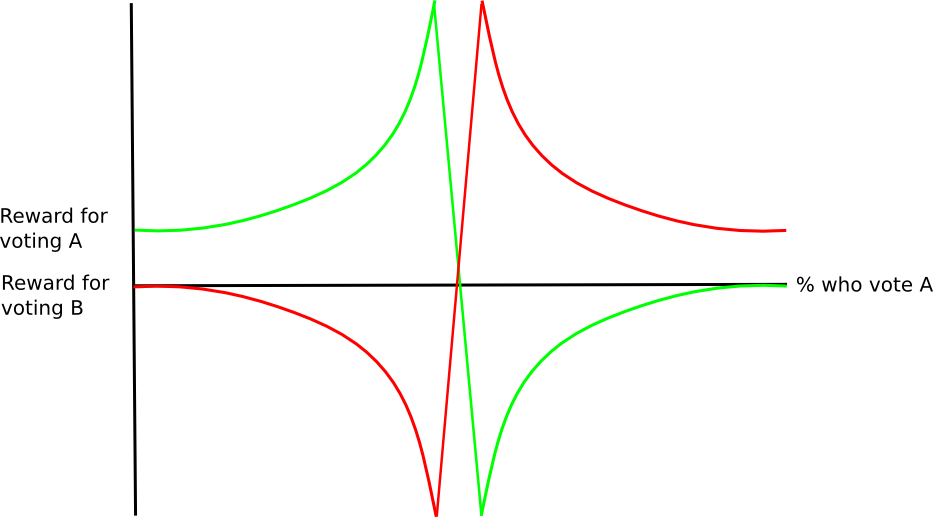
\includegraphics[width=165pt]{schellingcoin_payoff1.png}
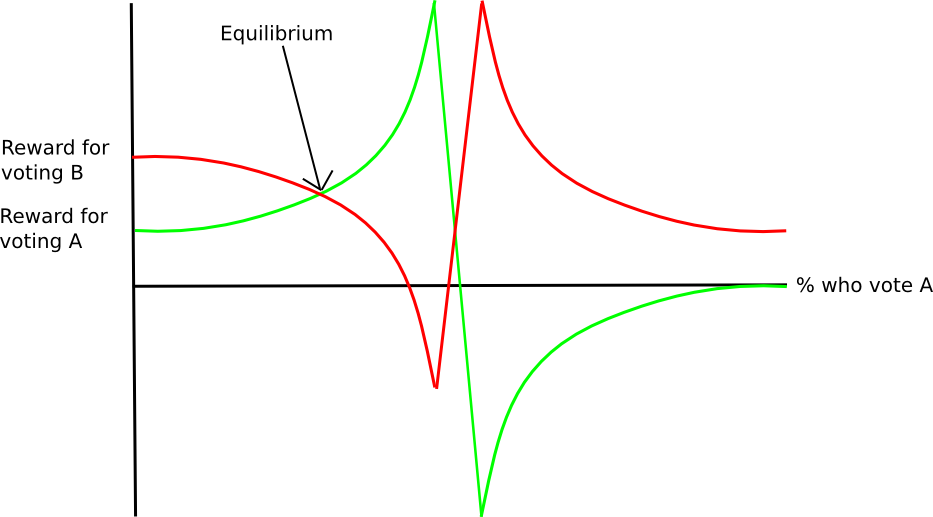
\includegraphics[width=165pt]{schellingcoin_payoff2.png}
\end{center}

This approach accepts that attackers with a budget even larger than the size of everyone's security deposits will be able to cause everyone to flip to voting incorrectly as an equilibrium, but advocates note that attackers that large will also be able to arbitrarily disrupt the underlying blockchain consensus anyway.

The second is to fall back to ``subjective resolution'': if the majority of voters vote incorrectly, then it is up to \emph{the users} to simply reject that block as invalid and go along with the block that they see as correct. This reliance on human judgement at the last level makes the budget required for any kind of zero-cost ``equilibrium flip'' attack essentially infinite, instead requiring the attacker to bribe everyone outright and even then resulting in only a moderately large inconvenience for users, not a total failure. The process does impose inconveniences to users, but properly built designs that use decentralized oracle schemes will use the mechanism only as the last step of a fallback game in a similar function as nuclear deterrence; in practice it will almost never be used. The security claim essentially becomes something like ``by paying \$100 million, an attacker has the ability to force users to visit their favorite internet forum and locate a 32-byte hash representing the new fork of the chain to switch to''.
\end{note}

\begin{defn}[Distributed hash table]
A distributed hash table is a mechanism which gives network-connected nodes access to a function $GET(\rho, i) \rightarrow (V, \pi)$ where $(V, \pi)$ is the Merkle branch of $\sigma[i]$ where $\rho = R(\sigma)$. $GET$ should work with overwhelmingly high probability provided that (i) $(V, \pi)$ has at least once been in the hands of at least one altruist, and (ii) the total quantity of data stored in the DHT is at most $\frac{N * n}{k}$ where $N$ is the computational and data storage capacity of a node, $n$ is the number of nodes and $k$ is a constant.
\end{defn}

\begin{note}
The Merkle-branch-based definition of DHT given above can be deduced easily from the more conventional definition of providing a function $GET(h) \rightarrow x$ where $h = H(x)$ for some hash function, given that Merkle tree protocols consist simply of repeated reverse-hash-lookup queries. The definition used above is more relevant to our ``scalable blockchain'' use cases.
\end{note}

\begin{exmp}
Kademlia \cite{kademlia} is an example of a distributed hash table. A more direct implementation of our desired formalism with Merkle branches will be available from IPFS \cite{ipfs}.
\end{exmp}

\chapter{Global Variables}

In the rest of this document we will use the following variables:

\begin{itemize}
\item
$N$ - the maximum computational power of a node
\item
$L$ - the level of economic activity in the network
\item
$m$ - the size of the randomly selected pool of validators that need to validate each block (usually 50 or 135)
\item
$w_a$ - the portion of weight controlled by altruists
\end{itemize}

$\tau$ will represent transactions, $\beta$ will represent blocks and block headers depending on context, and $B$ will represent ``super-blocks''.

\chapter{A Byzantine-fault-tolerant Scalable Consensus Algorithm}

Suppose a construction where the state is partitioned into $n \in O(N^{1-\epsilon})$ substates, and each substate is itself partitioned into very small parts (eg. one per account). We define three ``levels'' of objects:

\begin{itemize}
\item
A \emph{super-block} is a block in the top-level consensus process. The \emph{header chain} is the blockchain of super-blocks.
\item
A \emph{block} is a package containing:

    \begin{itemize}
    \item
    $T$, a list of transactions
    \item
    $D$, the set of Merkle branches for the observed area of T on the fine-grained sub-partition level, ie. where the value proven by each Merkle branch is only constant-size
    \item
    A \emph{header}, consisting of:
        \begin{itemize}
        \item
        $AP$, a map $\{i: R(\sigma[i]) \; for \; i \in OBSERVED(\sigma, T)\}$
        \item
        $AN$, a map $\{i: R(\sigma'[i]) \; for \; i \in OBSERVED(\sigma, T)\}$
        \item
        $S = [s_1 ... s_m]$, an array of signatures
        \item
        $H(T)$
        \item
        $H(D)$
        \end{itemize}
    \end{itemize}
\item
A \emph{transaction} is a transaction as before.
\end{itemize}

We use any non-scalable consensus algorithm (eg. Tendermint\cite{tendermint}) for processing super-blocks, except that we define a custom ``top-level'' state transition function $APPLY'$. For the state processed by $APPLY'$, we use $\psi = \{i: R(\sigma[i]) \; for \; i \in [n]\} + E(\sigma) + V(\sigma)$ where $E(\sigma)$ is a cryptoeconomically secure entropy source in $\sigma$ and $V(\sigma)$ is a set of ``validators'' registered in $\sigma$. From the point of view of $APPLY'$, we define a block header $\beta$ as being valid in the context of $\psi$ if the following are all true:

\begin{itemize}
\item
For all $i \in AP$, $\psi[i] = AP[i]$.
\item
For at least $\frac{2m}{3}$ values of $i \in [m]$, $s[i]$ is a valid signature when checked against $SAMPLE(W, E(\sigma) + A, m)[i]$ where $W(\sigma, u_i) = \frac{1}{|V(\sigma)|} \; if \; u_i \in V(\sigma) \; else \; 0$ and $A$ is the address or public key of the block proposer (ie. the block has at least $\frac{2m}{3}$ valid signatures out of a randomly selected pool of $m$).
\end{itemize}

If $\beta$ is valid, we set $\psi'$ by:

\begin{itemize}
\item
For all $i \in OBSERVED(\sigma, \beta)$, $\psi'[i] = AN[i]$
\item
For all $i \notin OBSERVED(\sigma, \beta)$, $\psi'[i] = \beta[i]$
\end{itemize}

The top-level state transition function has an additional validity constraint: for the super-block to be valid, the observed areas of all $\beta[i]$ must be disjoint from each other.

We do not formally put it into the top-level validation protocol, but we separately state that a validator is only supposed to sign a block if the block meets what we will call \emph{second-level validity criteria} for $\beta$:

\begin{itemize}
\item
Every transaction in $T$ is valid in its context when applied to $\sigma$.
\item
$D$, $AP$, and $AN$ are produced correctly.
\end{itemize}

\begin{lem}
Assuming less than $\frac{1}{3}$ of validators are Byzantine, a block that is valid under the above top-level state transition function will produce a top-level state $\psi'$ such that if we define $\sigma'$ with $\sigma' = \{i: R^{-1}(\psi'[i])\}$, $\sigma' = \sigma + T_1 + T_2 + ...$ where $T_i$ is the set of transactions in $\beta_i$.
\end{lem}

\begin{proof}
Suppose that all $\beta_i$ satisfy the second-level validity criteria. Then, note that each substate in $\sigma$ is only modified by at most one $T_i$, and so we can model the state as a tuple $(O, A_1, A_2, A_3 ... A_n)$ if $\beta$ includes $k$ transactions, where $A_i$ is the affected area of $T_i$ and $O$ is the remaining part of $\sigma$. The state after $T_1$ will be $(O, A'_1, A_2, A_3 ... A_n)$, by disjointness the state after $T_2$ will be $(O, A'_1, A'_2, A_3 ... A_n)$, and so forth until the final state is $(O, A'_1, A'_2, A'_3 ... A'_n)$. If we use the top-level state transition function on $\psi$, we can partition $\psi$ similarly into $(O, B_1, B_2, B_3 ... B_n)$, and a similar progression will take place, with state roots matching up at every step. Hence the final state at this top-level state transition will be made up of the roots of the substates in $\sigma'$.

Now, suppose that one $\beta_i$ does not satisfy the second-level criteria. Then, validators following the protocol will consider it invalid, and so $\frac{2m}{3}$ validators will not be willing to sign off on it with very high probability, and so the block will not satisfy the top-level criteria.
\end{proof}

Hence, we know that the resulting $\psi'$ will represent a state which is \emph{valid}, in the sense that it can be described as a series of transactions applied to the genesis. This is the validity criterion that we will repeatedly use in order to prove that validity is preserved by other mechanisms that we introduce such as revert mechanics.

Because a sampling scheme is inherently probabilistic, it is theoretically prone to failure, and so we will precisely calculate the probability that the protocol will fail. Assuming a 96-bit security margin, we can consider a probability negligible if the average time between failures is longer than the time it takes for an attacker to make $2^{96}$ computations. If we assume that the cryptoeconomically secure entropy source updates every super-block, and a super-block comes every 20 seconds, then one can reasonably expect a hostile computing cluster to be able to perform $2^{48}$ work within that time, so we will target a failure probability of $2^{-48}$ (this implies roughly one failure per 445979 years of being under attack). We can determine the failure probability with the binomial distribution formula:
\\
\\
$PE(n, k, p) = p^k * (1-p)^{n-k} * \frac{n!}{k!(n-k)!}$
\\
\\
Where $PE(n, k, p)$ is the probability of an event that occurs with probability $p$ in an attempt will achieve exactly $k$ occurrences out of $n$ attempts. For convenience, we define $PGE(n, k, p) = \sum_{i=k}^n PE(n, i, p)$, ie. the probability of \emph{at least} k occurrences.

We note that $PGE(135, 90, \frac{1}{3}) = 2^{-48.37}$, so 135 nodes will suffice for a $k = \frac{1}{3}$ fault tolerance. If we are willing to lower to $k = \frac{1}{5}$, then $PGE(39, 31, \frac{1}{5}) = 2^{-48.58}$, so 39 nodes will be sufficient. Additionally, note that if we want greater efficiency under normal circumstances, then a bimodal scheme where either 44 out of a particular 50 nodes ($PGE(50, 44, \frac{1}{3}) = 2^{-49.22}$) or 90 out of a particular 135 nodes is a sufficient validity condition will allow the cheaper but equally safe condition to work in the (usual) case where there are almost no malicious nodes, nearly everyone is online and the network is not under attack, and fall back to the more robust but bulkier validation rule under tougher conditions.

Additionally, note that the combinatoric formula is only valid if the entropy used to determine validator sets is \emph{actually} random, or at least close enough for our purposes. For this, our second uninfluenceability criterion, stipulating that an attacker with less than $\frac{1}{3}$ of all validators will be able to influence it by at most a reasonably small linear amount (in the NXT case, by a factor of $\frac{3}{2}$), is crucial, showing that with such a powerful attacker the probability of a successful attack remains below $2^{-47.4}$. The first uninfluenceability criterion is important in order to avoid excessive superlinear returns resulting from super-block proposers manipulating the entropy in order to increase the chance that their validators will be involved in verifying blocks, but does not affect security.

To see the role of the unpredictability criterion, note that the protocol as described here provides \emph{ex ante} Byzantine fault-tolerance, but not \emph{ex post} Byzantine fault tolerance; \emph{after} the validators are selected, only that small fixed number of validators acting maliciously will compromise the system. If entropy becomes unpredictable very slowly (or never at all), then the algorithm is only Byzantine fault-tolerant against faults very far in advance, leading to potential practical vulnerabilities like an attacker locating the 135 validators that will be validating their block one year from now and taking the time to locate and hack into 90 of them.

\begin{lem}
The above protocol is scalable.
\end{lem}

\begin{proof}
The load of a validator consists of two parts:

\begin{itemize}
\item
validating the header chain
\item
validating the blocks
\end{itemize}

For the header chain, note that the size of each super-block is $n+k_1b+k_2$, where $n$ is the size of the state partition (as each index can be included as an observed area at most once), $b$ is the number of blocks, $k$ is a constant representing the size of $H(T) + H(D) + [s_1 ... s_m]$, and $k_2$ is a constant for miscellaneous super-block data (eg. validators entering and leaving, the entropy source, timestamp, previous block hash). We can require $n \in O(N^{1-\epsilon})$ and $b \le n$ so $b \in O(N^{1-\epsilon})$. One can come up with an algorithm to evaluate the top-level validity of the block in less than $O(N)$ time; showing that observed areas do not intersect as a set non-intersection algorithm can take up to $O(k*log(k))$ time for $k$ items and $O(N^{1-\epsilon} * log(N^{1-\epsilon})) < O(N)$, and the individual block validations should simply take $O(N^{1-\epsilon})$ time.

For block validation, suppose that there are $v \in O(N^{1-\epsilon})$ validators. Each super-block may contain a maximum of $n$ blocks, and $n \in O(N^{1-\epsilon})$. Thus, in total, validators must process at most $m*n$ blocks (as each block must be processed by $m$ validators), and so each validator will on average end up processing $m*n/v \le O(1)$ blocks. If each block has $O(N^{1-\epsilon})$ transactions, then the computational load of this is $m * O(N^{1-\epsilon}) < O(N)$. Hence, the total load of a validator is less than $O(N)$ while the network processes a total of $O(N^{2-\epsilon})$ transactions.

From a bandwidth perspective, the header chain is sent to everyone, but for blocks the block proposer need only send the block to the validators directly, so once again the load per validator is $O(N^{1-\epsilon})$. The only data that a validator needs to verify the block is the observed areas on the sub-partition level, which are provided with proofs inside of $\beta$.
\end{proof}

The incentives inside such a scheme would be provided as follows:

\begin{itemize}
\item
Transactions can pay transaction fees to the producer of the block that includes them.
\item
Blocks can pay transaction fees to the proposer of the super-block that includes them, as well as the the validators that will sign off on them.
\item
The proposer of the super-block can pay transaction fees to the validator pool of the super-block; this fee can be mandatory (ie. protocol-enforced) or enforced by validators refusing to sign a block with a fee that is too small for them.
\item
The protocol may optionally add a mandatory fee to transactions and blocks, and this fee can get destroyed. The protocol may also add an \emph{ex nihilo} reward to the validators of the super-block in place of requiring it to be paid from transaction fees.
\end{itemize}

We can also require validators to have security deposits of size $O(N^{1-\epsilon})$ which are destroyed if the validators are malfeasant, as is standard in modern proof-of-stake consensus schemes; this provides the basis for an economic security margin. Note that the fees paid to validators, as well as the deposit size of a validator, is stored in the header chain alongside the identity of the validator; only when a validator leaves the pool does the fee balance get added to the main state.

\chapter{Fallback Schemes}

The previous algorithm provided a statistical guarantee of data availability and validity by simply assuming that at least two thirds of validators are honest; however, it carries an inherent fragility: if, for any reason, a small sample of nodes actually does end up signing off on an invalid block, then the system will need to hard-fork once the fault is discovered. This results in two practical weaknesses. First, larger safety factors are required on the sample sizes in order to ensure that a sample is absolutely never malicious. Second, the economic security of the algorithm, under our formal definition, approaches zero as $L$ increases if defined as a fraction of $L$. An attacker will only need to bribe $m$ out of a total $O(N^{1-\epsilon})$ validators in order to produce an invalid block that enters the system. Hence, as $N$ increases, there is no fixed bound $b$ of proportionality between the weight and the security margin; the ratio goes lower the larger the system gets. Sampling provides security against random faults, but not against targeted faults, which bribery can theoretically achieve.

One approach to dealing with the latter issue is to not bother with economic security, and simply rely on Byzantine-fault-tolerance guarantees to determine security. In order to ensure beneficence of the network maintains over time, we ask validators to censor attempts to join the validator pool by parties that appear to be unreliable or likely to be malfeasant. In some cases, particularly regulated financial systems, such restrictions are necessary in any case and so we need to go no further\cite{swanson}. If we are trying to create a more open network, however, then such a solution is unsatisfactory, and so we arguably need not just Byzantine fault tolerance but also regulation via economic incentives.

If economic security is indeed desired, one natural solution that may be proposed is a ``fallback game'': allow any validator to ``challenge'' a particular block's validity by putting some quantity of funds at stake (if no funds are at stake, then an attacker can increase load on the network arbitrarily at no cost), and ask the header chain to be the ``validator-of-last-resort''. If the data for the block is available, then this is easy: the validator provides the full block to the header chain, and the header chain validates the block; if the block is valid, then the challenger loses some portion of their security deposit, and if the block is invalid then the block is reverted and the validators that signed the block lose their entire security deposit (and a portion of that deposit goes to the challenger as a reward). The game that arises from this scenario can be seen as follows:

\begin{center}
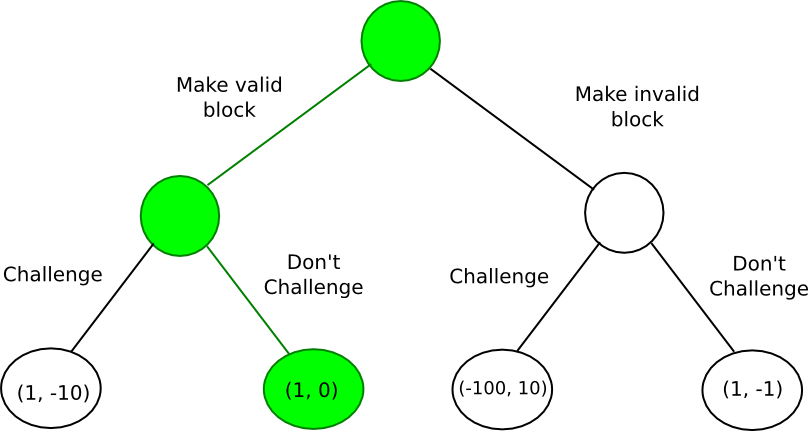
\includegraphics[width=200pt]{game.png}
\end{center}

Above we assume $1$ is the block reward, $-\delta$ is an expected private payoff to the validator of an invalid block getting into the blockchain (all we know about this payoff is that it is less than zero; it could take any magnitude depending on the situation of the particular validator and ultimately does not matter for the purposes of the game-theoretic argument), $100$ is the security deposit, $10$ is the whistleblower's reward and $-10$ is the penalty for whistleblowing falsely (ie. on a valid block). Note that the block producer ``plays'' first. If the block producer makes an invalid block, then the challenger will challenge, and so the block producer will earn $-100$; but by making a valid block the block producer will earn $1$. Hence, the block producer will make a valid block, and in that case the challenger will earn a higher profit of $0$ rather than $-10$ by not challenging and so will not challenge. Thus providing a valid block is a subgame-perfect equilibrium.

There are two problems with this scheme as described above. The first problem is a technical one: although the scheme remains scalable, Byzantine fault tolerant and economically secure, and even economically secure under a Byzantine failure or Byzantine-fault-tolerant under an economic attack, it is not \emph{scalable under an economic attack}. The reason is that an attacker can spend $\frac{L}{O(N^{1-\epsilon})}$ resources by bribing $m$ of the $O(N^{1-\epsilon})$ validators in order to elevate any block to the header level, and so by spending $b * L$ effort the attacker can elevate a total of $O(N^{1-\epsilon})$ blocks. As soon as the size of a block is at least $O(N^{2\epsilon})$ (which happens at $L \in O(N^{1+\epsilon})$), this means that by spending $b * L$ effort the attacker can make the protocol non-scalable.

The solution that we propose is a multi-round escalation game: a challenger proposes a transaction to point out an invalid previous block, and that transaction will be validated by $2m$ validators. If either the challenger or a validator is unhappy with the result, they can then make another challenge, providing twice as high a deposit but resulting in the block being reviewed by $4m$ validators. Another appeal is possible with a 4x deposit, which will be reviewed by $8m$ validators, and so on until all validators participate. Game-theoretically analyzing this, one can find that an attacker that spends $b * L$ resources can at most increase a node's computational load by a constant factor, and recursive elimination of dominated strategies leads to honesty being a subgame-perfect equilibrium in the normal case.

An alternative approach for ensuring validity is to simply use a succinct cryptographic proof in place of a cryptoeconomic one, seemingly removing the need for fallback schemes entirely. A zk-SNARK can theoretically be attached to the header of a block, proving that all of the transactions in the block are valid and that the final state roots are correct. However, this has a few problems. First, zk-SNARKs rely on much less robust cryptographic assumptions than hashes and signatures; particularly, it is not known if zk-SNARKs are even possible to secure against quantum computers, whereas strong candidates for quantum-proof digital signatures are well-known \cite{ntrusign} \cite{hashladder} \cite{sphincs}.

\chapter{Data availability}

The more difficult challenge in implementing a fallback scheme is that there are in fact two ways in which a block can be invalid. First, the block may incorrectly process transactions and have an invalid final substate root. Second, however, an attacker may simply create a (valid or invalid) block and refuse to publish the contents, making it impossible for the network to learn the complete final state. Validating data availability is, unfortunately, a fundamentally harder problem than validating correctness for a simple reason: data availability is quasi-subjective at scale. Although one can determine that a particular piece of data is available at a particular time by trying to download it, one cannot with perfect precision verify whether data is available if one does not have enough bandwidth to download all of it, and one cannot determine at all whether or not data was available at a previous time if one was not paying attention during that time.

A particular consequence of this is that validating data availability through cascading fallback, as described in the previous section above, is not so simple: the attacker can always cheat the system and destroy others' deposits by providing a block with unavailable data at first, waiting for a fallback game to start, and then destroying the security deposits of challengers by suddenly providing the data mid-game. Although such an attack does not compromise security, it does allow the attacker to siphon resources away from challengers, leading to an equilibrium in which it is not rational to challenge, at which point the attacker will be able to create and propagate bad blocks unimpeded.

In order to make clear the gravity of the problem, we will start off by showing several categories of attacks that are possible if data availability cannot be effectively ensured.

\begin{exmp}[Unprovable theft attack]
An attacker creates a block with transactions $T_1$ ... $T_n$, where $T_1$ ... $T_{n-1}$ are legitimate and applied properly but $T_n$ is an invalid transaction which seems to transfer \$1 million from an arbitrary wealthy user to the attacker. The attacker makes $T_1$ ... $T_{n-1}$ available, and makes the final state available, but does not make $T_n$ available. Once the state is confirmed by a sufficient number of future blocks, the attacker than spends the \$1 million to purchase other untraceable digital assets.

Here, note that there is no way to prove invalidity, because theoretically $T_n$ very easily \emph{could be} a transaction legitimately transferring \$1 million from the millionaire to the attacker, but the unavailability of the data prevents the network from making the judgement.
\end{exmp}

\begin{exmp}[Sudden millionaire attack]
An attacker creates a block with transactions $T_1$ ... $T_n$, where $T_1$ ... $T_{n-1}$ are applied properly but $T_n$ is an invalid transaction. The attacker then makes $T_1$ ... $T_{n-1}$ available, and makes \emph{most} of the final state available, with the exception of one branch where the attacker has given themselves \$1 million out of nowhere. Two years later, the attacker reveals this branch, and the network is forced to either accept the transaction or revert two years of history.
\end{exmp}

\begin{note}
One way to try to solve both attacks above is to require every valid transaction to show a valid ``source'' of its income. However, this leads to a recursive buck-passing problem: what if the attacker performs a sudden millionaire attack to create a new unexplained account $A_1$, then creates a block with an unavailable transaction sending funds from $A_1$ to $A_2$ (possibly a set of multiple accounts), then $A_3$, and so forth until finally collecting the funds at $A_n$, and then finally reveals all transactions upon receiving $A_n$. The total dependency tree of a transaction may well have total size $\omega(N)$. Peter Todd's tree-chains discussion offers the solution\cite{treechains} of limiting the protocol to handling a fixed number (possibly $\omega(N)$) of ``coins'', each one with a linear history; however, this solution is not sufficiently generalizeable and abstract for our purposes and carries high constant-factor overhead.
\end{note}

\begin{exmp}[Payment denial attack]
An attacker creates a block with an unavailable transaction which appears to modify another party's account (or spend their UTXO). This prevents the other party from ever spending their funds, because they can no longer prove validity.
\end{exmp}

\begin{note}
Even zk-SNARK protocols cannot easily get around the above problem, as it is information-theoretically impossible for any protocol regardless of cryptographic assumptions to fully specify the set of accounts that are modified in a particular super-block in $O(N)$ space if the set itself has $\omega(N)$ Kolmogorov complexity.
\end{note}

\begin{exmp}[Double-spending gotcha attack]
Suppose that a protocol tries to circumvent payment-denial attacks by making payment verification a challenge-response process: a transaction is valid unless someone can show that it is a double-spend. Now, an attacker can create a block containing a legitimate but unavailable transaction that spends \$1 million from account $A_1$ to $A_2$, also controlled by them. One year later, the attacker sends \$1 million from $A_1$ (which no one can prove no longer has the money because the data is unavailable) to $A_3$. One year after that, the attacker reveals the original transaction. Should the network revert a year of history, or allow the attacker to keep their \$2 million?
\end{exmp}

\begin{note}
Zk-SNARK protocols are not a solution here either, because of the same information-theoretic issues.
\end{note}

In order to remove the possibility of such issues in the general case, we will try to target a hard guarantee: given a general assumption that once data is available at all it is guaranteed to remain available forever due to a combination of the DHT and altruist-operated archival services, we will attempt to ensure that, for all blocks $\beta$, it is the case that either $\beta$ is available or $\beta$ is reverted.

The largest game-theoretic threat to fallback schemes handling the problem by themselves is, as discussed above, the ``crying-wolf attack'': an attacker repeatedly produces valid blocks with unavailable data, waits for a fallback process to start reverting them, and then immediately publishes the data, thereby discrediting the agents that contested the block in the eyes of all other viewers that did not have ther eyes on that particular block at the time that the incident was taking place. In order to prevent the process of contesting the block from becoming an attack vector, the process of contesting must be costly if it ends up being a false alarm; hence, eventually all challengers will be weary of wasting their resources, allowing the attacker to carry out unavailable-data attacks with impunity.

We can formally model this as follows, letting $c_c$ be the cost of raising a challenge, $r_c$ the reward of challenging successfully, $c_b$ the cost of producing an errant block, $c_v$ the cost of viewing a block, $B$ the block size, $n$ is the number of blocks and $n_v$ is the number of validators. 

\begin{itemize}
\item
We know that $n$ is proportional to $n_v$, since each validator can validate at most a fixed number of blocks.
\item
We know that $c_b$, $c_v$ and $B$ are proportional to each other, since the block size is proportional to $\frac{L}{n}$ where $n$ is the number of blocks, the cost of viewing a block is equal to the effort spent downloading it, and $c_b$ is bounded above by a validator deposit, which is also proportional to $\frac{L}{n}$. There is no reason to make $c_b$ less costly than needed, so setting $c_b$ to the entire deposit is prudent.
\item
We know that $c_c$ must be at least proportional to $\frac{L}{n} = B$, as otherwise an attacker of size $\epsilon * L$ would be able to repeatedly challenge every block. Note that $c_c$ is proportional to $B$ also allows an attacker of size $b' * L$ for some $b'$ to challenge every block; however, the degree of fallback escalation which the attacker can afford is bounded by a constant, whereas if $c_c < O(B)$ then the degree of escalation leads to a strictly complexity-theoretically greater level of attention on each block - and if this increased level was scalable then the protocol would have had it by default in the first place.
\item
We know that $c_r \le c_b$, as otherwise producing errant blocks and then calling them out would be a profitable strategy. Since $c_b$ is proportional to $B$, we know that $c_r$ is proportional to $B$.
\item
Hence, $c_c$ is proportional to $c_r$, so there is some constant $k = \frac{c_c}{c_r}$.
\item
A node starts off having some prior probability distribution $D$ over the probability $p$ of a random invalid block later revealing data. Assume for simplicity that this prior was derived from Laplacian succession\cite{laplace} with $s$ instances of later revelation and $f$ instances of non-revelation. After $f * k$ repeats of producing a block with invalid data and later revealing it, a node will rationally assume that the next block will have revelation probability $\frac{s + f * k}{s + f + f * k} > 1 - \frac{1}{k}$.
\item
Hence, it will not be rational for that node to issue a challenge when the next block with unavailable data appears.
\end{itemize}

This model is not intended to cover all possible scalable protocols - and indeed it can't, since we claim that there are in fact solutions; rather, it is intended to illustrate the general difficulty. Challenging this strategy requires irrational sacrifice of resources, either on the part of the challengers which would end up continuing to challenge blocks despite negative expected return or on the part of other actors that start issuing blocks with unavailable data without ever publishing the data purely in an attempt to manipulate challengers' posteriors \emph{in a positive direction}.

We provide two possible sets of solutions to this problem. The first is to simply capitulate to the crying-wolf attack, and explicitly require challenging to be a costly and potentially altruistic activity. The protocol in this case would work as follows:

\begin{itemize}
\item
After a block is published, initialize $i = 0$. Anyone has the ability to lay down a ``challenge'' against the block at cost $c$ within the next $F_d$ blocks (eg. $F_d = 20$). Challenging happens at the superblock level (ie. it is part of the top-level state transition function).
\item
Once at least $k * 2^i$ challenges are laid (eg. $k = 5$), the block enters ``purgatory''. Once in purgatory, the block remains there until it is either ``rescued'' (see below) or it remains there for $P_d$ blocks (eg. $P_d = 40$) at which point the block is reverted.
\item
Rescuing a block requires a ``rescue'' transaction, which requires signatures from two thirds of a random set of $2^{i+1} * m$ validators (eg. 180 of 270 at $i = 0$). This also happens at the superblock level, and the producer and validators of a successful rescue transaction are given a small reward (eg. $\frac{c}{3m}$ per validator plus $\frac{c}{3}$ to the producer).
\item
Once a block has been rescued, the $F_d$ time restarts, increment $i \leftarrow i + 1$, and the block can be challenged again. Note that each time the cycle repeats, the required number of challenges and the required number of validators on a rescue doubles.
\item
If a block is rescued by the entire network, then it can be considered final.
\item
If a block is challenged but never rescued, then the security deposits of the block producer and all validators that signed the block are destroyed, and equally split among challengers.
\end{itemize}

Under normal circumstances, challenging is thus profitable; it is only during a crying-wolf attack (which has a \emph{very} large constant-factor cost, perhaps even enough to make it not the weakest link in all but the largest $O(N^2)$ systems) that is becomes altruistic. Because anyone can challenge, one cannot bribe ``the challengers'' not to challenge; in fact, doing so will simply motivate the challenger to challenge again using a different identity. An attacker with at most $n * c$ resources can force at most $2 * n * m$ validators to check availability on a block, and so if we set $c \in N^{1-\epsilon}$, we can see that an attacker with $b * L \in O(N^{2-\epsilon})$ resources will be able to force $2 * m * O(N^{1-\epsilon})$ validators to check a single block, increasing their computational load by a constant factor; hence, the system cannot be subjected to a denial-of-service attack except at cost $b * L$ where the value of $b$ depends on $c$ (there is a linear tradeoff between requiring more altruism and being more susceptible to denial-of-service attacks).

We also add a rule that the producer of a block is slightly penalized if it is challenged sufficiently, even if it is later vindicated. This allows us to establish a bound on the ratio of losses to altruists to losses to the attacker, allowing a bound to be determined on the minimum required budget of an attacker assuming altruists are willing to lose $L * k * w_a$ for some constant $k$. Note that rescuing legitimately is a very low-risk activity; since a validator should possess the entire data of a block themselves, they have the ability to convince any larger sample of validity if necessary.

A possible scheme for removing the need for altruism even \emph{in extremis} works as follows. First, we require the proposer for each superblock to compute a small amount of proof of work, perhaps with per-superblock cost $w = r * 0.01$ where $r$ is the superblock reward. Proof of work is required to provide a highly secure cryptoeconomic entropy source which is completely unpredictable; alternatives such as NXT can far too easily be foretold in advance. From this value, we then select a random substate, and we ask all top-level validators to check availability on the most recent block in that substate. If the block is indeed unavailable, and the block has been challenged, then the challengers split a reward of size $r_c = w * 0.49 \in O(N^{2-\epsilon})$. The superblock proposer also gets a reward of equal size.

The scheme can be thought of an inverted application of a standard result from law and economics: one can achieve compliance with arbitrarily low enforcement cost by simply decreasing the level of enforcement, and thus the probability of getting caught, but simultaneously increasing the fine\cite{econofcrime} - except, in our case, we are performing the exact opposite task of a police department as we are trying to \emph{incentivize a virtuous usually-costly action} with the occasional application of a \emph{reward}. The load each validator is at most the cost of downloading one block, $O(N^{1-\epsilon})$, and each substate will have a propbbility of at least $\frac{1}{O(N^{1-\epsilon})}$ of being randomly inspected; hence the scheme does not compromise scalability. However, assuming that a top-level challenge has at least a fixed probability $p$ of correctly determining that an unavailable block is unavailable before the attacker manages to broadcast it across the network, this provides an average incentive of $\frac{r_c}{O(N^{1-\epsilon})} \in O(N)$ in order to challenge, making it statistically worthwhile to challenge invalid blocks despite the cost.

Note that it is expensive for the challenger to manipulate the proof of work either upward or downward. Once the challenger has computed the proof of work successfully, a bribe of size $r_c \in O(N^{2-\epsilon})$ is required to dissuade him from starting the top-level challenge procedure for the entire block, and with judicious choice of constants one can make the bribe exceed our desired threshold $b * L$. If the challenger wants to \emph{increase} the probability of triggering a top-level challenge in order to earn the $r_c$ reward, possibly in collusion with the challengers, then note that even if the attacker has placed an invalid block on \emph{all} substates, re-computing the proof of work has cost $w$ and maximum expected collective reward $w * 0.98$.

Given that the expected reward of challenging is now $\frac{w}{N^{1-\epsilon}}$, we can impose a cost of challenging of at most the same value, and so the level of denial-of-service protection we get against challenges is proportional to the quantity of proof of work employed. One can increase the ratio drastically at the cost of limiting ourselves to a more qualified security bound by setting $r_c = k * w$ for some $k > 1$, making proof-of-work manipulation profitable only if $\frac{1}{2k}$ of substates currently have an invalid block in them (due to the extreme cost of producing an invalid block, we can hence make $k$ quite high).

The second set of solutions to this problem involves changing the question asked to the fallback game: instead of asking the fallback game to adjudicate on the question of whether the data \emph{is} available, have it adjudicate on the question of whether the data \emph{was} available. This would then be combined with some kind of \emph{strategy} which each node would use to efficiently determine whether or not every challenge was valid as soon as it is made. There are two most promising contenders for such strategies. First, one can require the data of a block to be erasure coded, such that the data can be fully recovered if at least 50\% is available; this allows each node to probabilistically evaluate total availability by randomly accessing a sample (without erasure coding, a 99\% available block can easily slip through scrutiny). Second, one can require each node to independently pick a random sample of challenges to evaluate, and provide the Merkle root of the set of evaluations to other nodes. Other nodes would then probabilistically check the correctness of the Merkle roots that they receive through sampling, and would then themselves send out a Merkle root of all Merkle roots that they consider trustworthy. This can theoretically be made resistant to bribery because transmission of Merkle roots is private and so there is no way for a node to prove to a briber that they sent a compromised Merkle root.

For simplicity, we recommend not applying either of the more advanced strategies due to their greater complexity, and simply relying on altruism \emph{in extremis}, noting that in practice attempts to bribe validators have not proven to be a problem in cryptoeconomic systems in practice. If crying wolf attacks become a problem, particularly in the more highly scalable variants we describe in a later section, then we prefer the random block selection game due to its greater simplicity.

\chapter{Reverting}

A critical mechanism used in the previous sections is the concept of \emph{reverting} a block if it is found to be invalid. However, it is necessary to come up with a scheme to do so with minimal disruption, reverting only what needs to be reverted while keeping the remaining state transitions intact. To do so, we propose the following mechanism. When an invalid block is found and agreed upon, construct a ``dependency cone'' of all substates that could have been affected by that block, and revert each substate to a prior ``safe'' state. The algorithm for this relies on a primitive we will call $GDC$ (``get dependency cone''), which takes a target state $\sigma$, an errant block $\beta_0$ inside a super-block $B$ and the post-super-block state $\sigma_0 = \sigma_{-1} + B$, and outputs a partial mapping of index to substate. We define $GDC$ as follows:

\begin{itemize}
\item
$GDC(\sigma, \sigma_0, \beta_0) = \emptyset$ if $\sigma \in ANC(\sigma_0)$
\item
$GDC(\sigma_0, \sigma_0, \beta_0) = OBSERVED(\sigma_0, \beta_0)$
\item
$GDC(\sigma + B, \sigma_0, \beta_0) = \bigcup_{\beta \in B: GDC(\sigma, \sigma_0, \beta_0) \cap OBSERVED(\beta) \ne \emptyset} OBSERVED(\sigma, \beta)$ $\cup GDC(\sigma, \sigma_0, \beta_0)$
\end{itemize}

Assuming an invalid block $\beta_0$ inside a super-block $B$ with prior state $\sigma_{pre}$, and assuming the current state is $\sigma_f$, we use $GDC(\sigma_f, \sigma_{pre} + B, OBSERVED(\sigma_{pre}, \beta_0))$ to get the total set of substates to be reverted. Then, for each substate index $i$, we locate the state $\sigma_i$ such that $i \in GDC(\sigma_i + B, \sigma_{pre} + B, OBSERVED(\sigma_{pre}, \beta_0))$ but $i \notin GDC(\sigma_i, \sigma_{pre} + B, OBSERVED(\sigma_{pre}, \beta_0))$, and simply revert $\sigma'_f[i] \leftarrow \sigma_i[i]$, ie. revert every substate to just before the point where it got into the ``cone'' of potentially invalid blocks.

\begin{lem}
The state obtained after reverting as above is valid.
\end{lem}

\begin{proof}
For the sake of simplicity, suppose that every super-block contains a block modifying every substate; if not, then we assume a phantom ``null block'' for each unaffected substate $i$ with $AN = AP = \{i: R(\sigma[i])\}$. First, note that the area of the ``dependency cone'' during each super-block corresponds exactly to the combined area of some set of blocks; it cannot partially include any block because the definition states that if the area of a block is partially included it must be fully included, and it cannot include area unoccupied by blocks because of our siplifying assumption. Then, for each super-block $\beta$, let $D(\beta)$ be the set of blocks in the dependency cone of the post-state of that block in the blockchain, and $U(\beta)$ be the set of blocks not in the dependency cone. If $\sigma_f = \sigma_{pre} + \beta_1 + \beta_2 + ...$, the post revert state $\sigma'_f$ will correspond exactly to $\sigma_{pre} + U(\beta_1) + U(\beta_2) + ...$. 

We will show why this is true by illustration. Consider a sequence of states with a set of blocks updating the state during each super-block:

\begin{center}
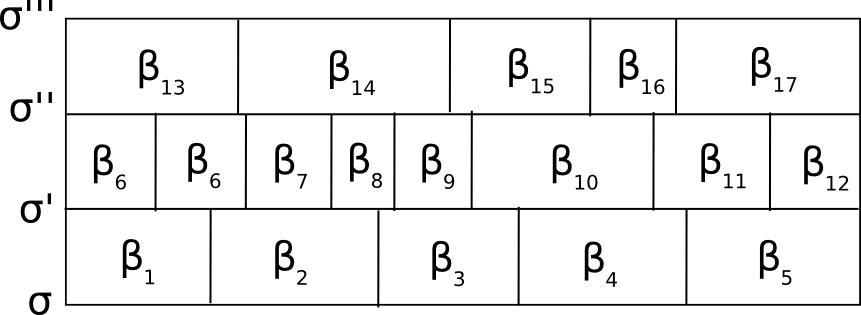
\includegraphics[width=200pt]{revert1.png}
\end{center}

Now, suppose that one of those blocks is invalid. Then, if we manage to revert immediately in the next block, the state will be moved to the red line here:

\begin{center}
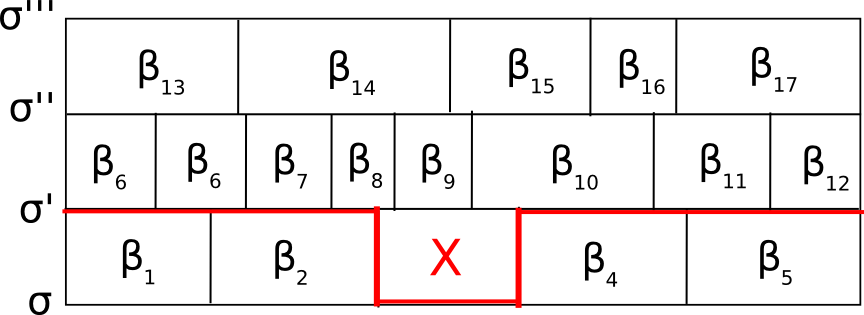
\includegraphics[width=200pt]{revert2.png}
\end{center}

And if we revert later, the state will be moved to the red line here:

\begin{center}
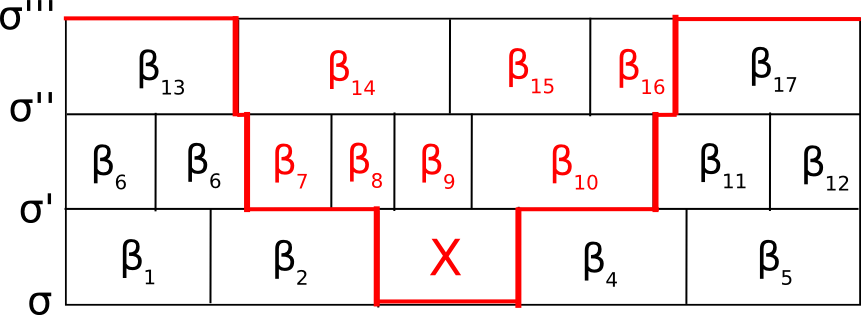
\includegraphics[width=200pt]{revert3.png}
\end{center}

Notice that one can apply the set of still-valid blocks sequentially to $\sigma$ to obtain $\sigma'_f$ in all cases.
\end{proof}

It is important to note that the revert process is scalable only if the number of substates that an attacker can revert with a single invalid block is bounded, assuming some bound on the amount of time that it takes for the bad block to be detected and for the revert to be included. Otherwise, the attacker can annoy all users by paying less than $b * L$ cost, and so the algorithm will no longer be scalable under attack. In order to achieve this, we have two solutions. First, we can specify that each block can have a maximum area size $k$ for some fixed $k$; the number of substates reverted assuming a revert after $l$ blocks will then be bounded above by $k^l$. The other approach is to require blocks with area larger than $k$ substates to have proportionately more validators; eg. a block with area of size $4k$ substates should require $\frac{8m}{3}$ signatures out of a pool of $4m$ in order to be valid. Both strategies ensure scalability under attack.

\chapter{Stacking}

The above schemes provide scalability up to $O(N^{2-\epsilon})$. But can we go higher than that? As it turns out, the answer is yes; we can in fact achieve scalability of $O(N^{d-\epsilon})$ for arbitrary $d$ while satisfying both economic and Byzantine-fault-tolerance guarantees. We accomplish this by essentially layering the scheme on top of itself. Essentially, we define a generalized transform $T(APPLY, VT, N, d)$ where $APPLY$ is a state transition function, $VT(F, s) \rightarrow F'$ is a function which takes a state transition function $F$ and a maximum header chain size $s$ and outputs the top-level state transition function $F'$ (eg. the algorithms we defined above can be seen as implementations of $VT$), $N$ is the maximum computational load and $d$ is the depth.

We define $T$ as follows:

\begin{itemize}
\item
$T(APPLY, VT, 2) = VT(APPLY, N^{1-\epsilon})$
\item
$T(APPLY, VT, d) = T(VT(APPLY, N^{d*(1-\epsilon)}), VT, d-1)$ for $d > 2$
\end{itemize}

We maintain the restriction that all objects produced at any point must have a soft maximum size, above which the number of validators required to agree on that object increases proportionately.

The definition is simple, and so somewhat obscures the complex inner workings of what is going on. Hence, let us provide an example. Consider a transform of the fallback-plus-subjective-resolution scheme provided above with $d = 3$. There would now be four ``levels'' of data structures. At the bottom level, we have the ultimate transactions that are affecting the state. Then, on the third level we have blocks containing those transactions. To validate blocks on this third level, there are $O(N^{2-\epsilon})$ validators (each with a deposit of size $O(N)$), which are recorded on the second level; a block on the third level must obtain signatures from $\frac{2m}{3}$ out of a pool of $m$ validators obtained from \emph{the entire pool} of second-level validators. However, the process of verifying that signatures from the correct validator pool are provided itself depends on data that is not shared globally (as it is on the second level), and so that process itself as a state transition function needs to be carried out using the two-level scalable protocol, ie. a second-level block would treat the second-level validators accessed by all third-level blocks contained inside of it as part of its ``observed area''. Blocks containing these transactions would themselves be voted on by the header chain, which has $O(N^{1-\epsilon})$ validators each with a deposit of size $O(N^2)$.

\begin{center}
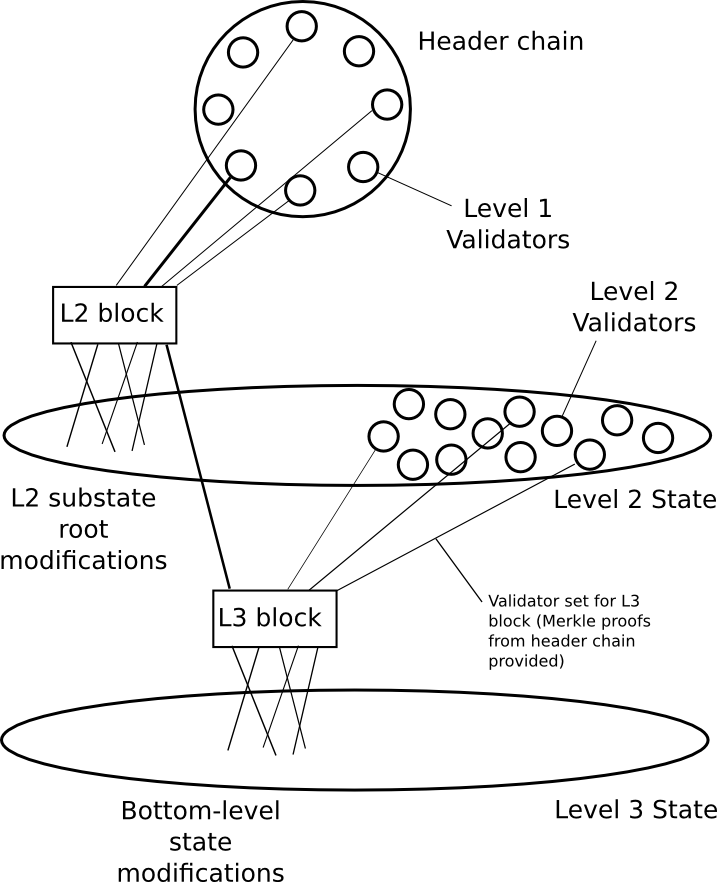
\includegraphics[width=250pt]{multilevel.png}
\end{center}

At this point, the algorithm almost has $O(N^{3-\epsilon})$ scalability, but not quite. There are two reasons why. First, note that each third-level block independently picks $m$ validators. Hence, if a second-level block has $O(N)$ transactions, and assuming that there are $O(N)$ second-level substates, we can expect a single second-level block to have an observed area of size $1 - \frac{1}{e^m}$ of the whole set of substates - which for even the highly unrealistic $m = 5$ amounts to almost all of it. Hence, there can be at most one second-level block, and so our scalability is right back to $O(N^{2-\epsilon})$.

To solve this problem, we make a moderate change: we say that the set of validators for any transactions should always be determined from the state \emph{at the start} of the super-block. Formally, we say that a superblock has two ``virtual transactions'' $\sigma \rightarrow (\sigma, \sigma)$ at the start, and then $(\sigma, \sigma') \rightarrow \sigma'$ at the end, and validators are selected from the left pool, not the right pool. This allows us to have validators be selected from anywhere in the state without including them into any observed areas. From an implementation perspective, this means that a block at any level would need to come with signatures $[s_1 ... s_m]$ and also Merkle proofs $[\pi_1 ... \pi_m]$ where $\pi_i$ proves that the validator $V_i$ that produced signature $s_i$ is indeed at the correct position in the validator pool of the super-block's pre-state.

Second, note that ``fallback'' mechanisms all eventually lead to \emph{all} validators in their validator pool processing a particular block, and producing a transaction which contains all of their signatures. Here, our largest validator pool is of size $O(N^{2-\epsilon})$, and so at least one node somewhere will have to process $O(N^{2-\epsilon})$ signatures. To solve this, we institute an additional rule: when the number of validators reached by a fallback scheme exceeds $O(N^{1-\epsilon})$, the next level of validation will return to $m$ validators, but \emph{one level higher}.

Now, consider the effort done at each level. In the header chain, we have $O(N^{1-\epsilon})$ validators, and each validator must on average perform top-level verification on $m$ blocks as before. On the second level, there would be $O(N^{2-\epsilon})$ validators, and there would be a total of $O(N^{2-\epsilon})$ blocks being produced, and so on average each validator would need to perform top-level verification on $m$ blocks. A second-level block producer would select an area $A$ of $k$ second-level substates, and fill the block with third-level blocks that have an effect inside that area; from the second-level validator's point of view, the third-level blocks look just like transactions would under an $O(N^{2-\epsilon})$ scheme, except with the difference that the validity condition requires verifying $m$ signatures. A third-level block producer would select an area of third-level substates, and fill the block with transactions that have an effect inside that area. Assuming the second-level block producer includes $O(N^{1-\epsilon})$ third-level blocks, and a third-level block producer includes $O(N^{1-\epsilon})$ transactions, all actors inside the system have less than $O(N)$ load.

Suppose that the scheme is attacked, by means of a successful invalid block with transactions at depth $d$ and header at depth $d - 1$. Then, challenges would be placed at depth $d - 1$, and eventually the block's time in purgatory would expire and the revert procedure would happen, reverting the substate roots at depth $d - 1$. The reversion process would itself require an object at depth $d - 1$ in order to process. Because the total economic volume is $O(N^{k-\epsilon})$, and there are $O(N^{d-\epsilon})$ validators at depth $d$, the cost of bribing $m$ validators at depth $d$ would be $m * N^{d - k}$, and the block would inconvenience roughly $O(N^{d - k})$ users, so a proportionality of attacker cost to network cost is maintained. The same escalation argument as before shows that the scheme does not become unscalable until the attacker starts making economic sacrifices superlinear in the economic activity in the blockchain.

In practice, we expect that the extra complexity in implementing such an ultra-scalable scheme will be sufficiently high that cryptoeconomic state machine developers will stick to simpler two-level scaling models for some time. However, the result is important as it shows that, fundamentally, the level of overhead required in order to have a blockchain of size $L$ is roughly $m * log(L)$, a very slowly-growing value. With clever use of zk-SNARKs, perhaps even a completely constant-overhead approach for blockchains of arbitrary size can be achieved.

\chapter{Strategy}

The above sections described the \emph{algorithms} that can be used to convert a state transition function into validity criteria that can be used in order to build a scalable blockchain architecture out of traditional non-scalable components. However, there is also a need to develop higher-level \emph{strategies} that would be used by validators in order to allow a maximally expressive set of state transitions to effectively execute.

One major category of strategy that must be developed is for \emph{index selection}. Each block producer must determine what set of substate indices they will be keeping up to date on the state for, and be willing to produce blocks containing. In the event that transactions requiring a larger area appear, the groups of block producers will likely need to somehow cooperate in order to be able to produce a block containing the combined area. One possible strategy is for validators to arrange substate indices in a k-dimensional space, and maintain up-to-date knowledge of $\sigma[i]$ for either a radius-r cube or at least two adjacent substates. An alternative approach, specialized to simpler state transition functions involving sending from A to B (such as that of Bitcoin), is to maintain $(i, j)$ pairs and update $i$ and $j$ often. A third approach is adaptive: use some kind of algorithm to determine which substate indices appear together most often, and try to keep track of an increasingly contiguous cluster over time. If transaction senders also adapt their activities to substate boundaries, the co-adaptation process can potentially over time create highly efficient separations.

Additionally, note that index selection also becomes a concern when one or more blocks is in purgatory. In this case, a block producer producing a block on top of a block in purgatory has the concern that their block may be reverted. Hence, a possible strategy that block producer may employ in that case is to compute the dependency cones of all presently challenges blocks, and refuse to produce blocks that are fully or partially inside any such dependency cone. In that case, however, the block producer may also wish to check availability on the contested block themselves, and if it is contested create a rescue transaction.

The other category of strategy is for transaction sending, particularly in the context of more complex state transition functions like that used in Ethereum. If a transaction only affects a few neighboring substates, then an index selection strategy as above will be able to provide easy and global transfer. However, what happens if an action needs to be performed that has wide-reaching effect, and it is impractical to put it into a single block? In this case, one option is to set up an ``asynchronous routing'' meta-protocol: if a transaction affects state $\sigma[i]$ but also needs to effect a change in $\sigma[j]$, then if it is acceptable for the latter change to be asynchronous we can have a message be passed through a ``network'' of contracts, first to a contract in a state neighboring $\sigma[i]$, then hopping progressively closer to $\sigma[j]$ during subsequent transaction executions until finally arriving at $\sigma[j]$ and effecting the desired change. Note that this is equivalent to the hypercubes \cite{hypercubes} strategy developed for Ethereum in 2014; but instead of being a core part of the protocol, the protocol has been abstracted even further out allowing hypercubes to simply be one of the many possible strategies that the protocol can lead to.

If the primary purpose of a blockchain is to act as a currency system, then as long as sufficient liquidity exists one can get by with a very low amount of interoperability. For example, even if it is only possible to move funds between substates every 1000 blocks, and even then only through a single central ``hub state'' (which is assumed all nodes store as a strategy), that limited movement provides enough fungibility for the currency units in the various substates to maintain fungibility. Cross-substate payments can be done by means of various decentralized exchange protocols, treating the different substates as different currencies with the only difference being that the currency exchange rate will always remain equal to 1. However, it is debatable whether this approach is preferable to the other strategy described above of having block proposers select random $(i, j)$ pairs.

Finally, there is the protocol-level decision of how to maintain the divisions between substates and grow and shrink the total number of substates if necessary. There are several categories of solution here:

\begin{itemize}
\item
Employ an adaptive algorithms, perhaps adapting Karger's minimal-cut algorithm \cite{karger}, in order to split and join substates over time. Note that this can be done at the strategy level, giving the top-level consensus the right to split and join substates arbitrarily, but making it economically efficient for them to make splits that create a minimal cut. One disadvantage of this approach is that if transaction fees are priced so as to disincentivize cross-substate activity, fees for specific operations become unpredictable since substates can be rearranged.
\item
Create new substates every time existing substates get too large, and incentivize users that marginally care less about network effect to act in those substates by lowering transaction fee pricing. This removes the ability to make arbitrary splits, but also leads to unpredictable pricing since prices do need to go up to incentivize users away from high-activity substates - although the pricing would be far more even and less discretionary.
\item
Allow users to set the location of objects in the state with arbitrary fineness, but with increased cost for higher degrees of fineness. Hence, objects that need to be very close to each other can pay the cost for extreme co-location, whereas other objects can place themselves further apart. This is the strategy undertaken in Gavin Wood's fiber-chains proposal\cite{fiberchains}.
\end{itemize}

\chapter{Further optimizations}

The algorithms described above are meant to be starting points, and are by no means optimal. The primary areas of optimization are likely to be fourfold:

\begin{itemize}
\item
Reducing the limits imposed on state transition functions while maintaining identical levels of scalability
\item
Achieving constant-factor gains by increasing efficiency of Merkle proofs, block sending protocols, safely reducing the value of $m$, reducing churn, etc.
\item
Increasing block speed
\item
Making reverts less harmful by using inclusive blockchain protocols (ie. if $\beta_1 ... \beta_n$ is the set of blocks that was reverted, and $\sigma'_f$ is the post-revert state, automatically update to $\sigma''_f$ = $\sigma'_f {++} \beta_1 {++} ... {++} \beta_n$).
\item
Providing the option for even higher gains of efficiency but at the cost of less-than-perfect guarantees of atomicity, ie. reducing $m$ to $8$ with the associated cost gains but with the understanding that the action happens within a cordoned-off area of the state where invalid transitions will sometimes happen.
\end{itemize}

For the first of these, the most promising direction where one can find easy immediate gains is to try to separate observed area from affected area. Theoretically, there is no interference risk if two blocks in a super-block share observed areas, as long as that observed area is not any block's affected area. The challenge is (i) figuring out what hard limits to impose on a block in order to make sure that the scheme remains scalable (eg. if there are $\frac{n}{2}$ blocks each using $\{\frac{n}{2}+i\}$ as their observed area and $[\frac{n}{2}]$ as their observed area, the super-block will have $\frac{n^2}{4}$ hashes and will thus be unscalable), and (ii) figuring out how to manage reverts.

If one wants to go even further, one can allow the affected area of one block to be the observed area of another block, as long as one can arrange all blocks in an order such that each block is observed before it is affected. But there is a fundamental tradeoff between expressivity and fragility: the more the state transition function is able to process synchronous updates of very many and arbitrary states, the more costly a successful attack becomes if it must be reverted.

For the second, the largest tradeoff is likely to be that between churn and security. If one can keep the same $m$ nodes validating the same substates for a longer period of time, eg. half an hour, one may be able to reduce network load. However, keeping a constant pool for too long makes the scheme more attackable.

For the third, the most likely source of gains will be improvements in the underlying non-scalable consensus algorithm used to maintain consensus on the top-level state $\psi$. Inclusive blockchain protocols such as those developed by Sompolinsky and Zohar \cite{inclusive} are a potential route for minimizing disruption under ultra-fast block times, and such protocols can also be used for the fourth goal of mitigating the impact of reverts.

For the fifth, an ideal goal would be to have a blockchain design which allows users to pick a point on the entire tradeoff space between cost and probability of failure, essentially capturing in the base protocol concepts like ``auditable computation'' \cite{auditable} (where computation is done by a third party by default, but if an auditor finds the third party provided an incorrect result the auditor can force the execution to be re-done on the blockchain and if the third party is indeed in the wrong it loses a security deposit from which the auditor will be able to claim a bounty).

Finally, there is plenty of room for optimization in strategies, figuring out how validators can self-organize in order to maximize the expressivity of the state transition function in practice. The ideal goal is to present an interface to developers that ``just works'', providing a set of highly robust abstractions that achieve strong security bounds, freeing developers of the need to think about the underlying architecture, math and economics of the platform unless absolutely necessary. But this problem can be solved much later than the others, and solutions can much more easily continue to be iterated even after the underlying blockchain protocol is developed.

\begin{thebibliography}{32}

\bibitem{mmpetertodd}
    Peter Todd on merge-mining, Dec 2013: \url{http://sourceforge.net/p/bitcoin/mailman/message/31796158/}

\bibitem{coiledcoin}
    What is the story behind the attack on CoiledCoin? (StackExchange, 2013): \url{http://bitcoin.stackexchange.com/questions/3472/what-is-the-story-behind-the-attack-on-coiledcoin}

\bibitem{parallelcomputing}
    Amdahl and Gustafson's laws and Bernstein's conditions for parallelizability (Wikipedia): \url{http://en.wikipedia.org/wiki/Parallel_computing#Amdahl.27s_law_and_Gustafson.27s_law}

\bibitem{gmaxwell}
    Gregory Maxwell and jl2012, Bitcointalk: \url{https://bitcointalk.org/index.php?topic=277389.45;wap2}

\bibitem{auditable}
    Scalability, Part 1: Building on top, Vitalik Buterin, September 2014: \url{https://blog.ethereum.org/2014/09/17/scalability-part-1-building-top/}

\bibitem{lightning}
    Lightning Network: \url{http://lightning.network/}

\bibitem{zamfir}
    Vlad Zamfir's Formalizing Decentralized Consensus, coming soon.

\bibitem{piketty}
    Thomas Piketty, Capital in the 21st Century: \url{http://www.amazon.com/Capital-Twenty-First-Century-Thomas-Piketty/dp/1491534656}

\bibitem{bar}
    BAR Fault Tolerance for Cooperative Services, Amitanand S. Aiyer et al: \url{http://cs.brown.edu/courses/csci2950-g/papers/bar.pdf}

\bibitem{amiller}
    Anonymous Byzantine Consensus from Moderately-Hard Puzzles: A Model for Bitcoin, Andrew Miller, Joseph J LaViola Jr: \url{https://socrates1024.s3.amazonaws.com/consensus.pdf}

\bibitem{merkle}
    Merkle trees (Wikipedia): \url{http://en.wikipedia.org/wiki/Merkle_tree}

\bibitem{kademlia}
    Kademlia: A Peer-to-peer Information System Based on the XOR Metric \url{http://pdos.csail.mit.edu/~petar/papers/maymounkov-kademlia-lncs.pdf}

\bibitem{ipfs}
    IPDS: \url{http://ipfs.io/}

\bibitem{zamfirpoc}
    Vlad Zamfir and Pavel Kravchenko's Proof of Custody: \url{https://docs.google.com/document/d/1F81ulKEZFPIGNEVRsx0H1gl2YRtf0mUMsX011BzSjnY/edit}

\bibitem{ffterasurecode}
    $O(N*polylog(N))$ Reed-solomon erasure codes via fast Fourier transforms: \url{http://arxiv.org/pdf/0907.1788.pdf}

\bibitem{nxtinside}
    nxtinside.org, describing the NXT generation signature algorithm: \url{http://nxtinside.org/inside-a-proof-of-stake-cryptocurrency-2/}

\bibitem{snark}
    Succinct Zero-Knowledge for a von Neumann Architecture, Eli ben Sasson et al, Aug 2014: \url{https://eprint.iacr.org/2013/879.pdf}

\bibitem{schellingcoin}
    SchellingCoin: A Zero-Trust Universal Data Feed, Vitalik Buterin, Mar 2014: \url{https://blog.ethereum.org/2014/03/28/schellingcoin-a-minimal-trust-universal-data-feed/}

\bibitem{pepsilon}
    The P + Epsilon Attack, Vitalik Buterin, Jan 2015: \url{https://blog.ethereum.org/2015/01/28/p-epsilon-attack/}

\bibitem{sztorc}
    Truthcoin: Trustless, Decentralized, Censorship-Proof, Incentive-Compatible, Scalable Cryptocurrency Prediction Marketplace, Paul Sztorc, Aug 2014: \url{http://www.truthcoin.info/papers/truthcoin-whitepaper.pdf}

\bibitem{tendermint}
    Tendermint: Consensus without mining, Jae Kwon: \url{http://tendermint.com/docs/tendermint.pdf}

\bibitem{swanson}
    Permissioned Distributed Ledger Systems, Tim Swanson: \url{http://www.ofnumbers.com/wp-content/uploads/2015/04/Permissioned-distributed-ledgers.pdf}

\bibitem{ntrusign}
    NTRUSign: Digital Signatures Using The NTRU Lattice, Jeffrey Hoffstein et al: \url{http://www.math.brown.edu/~jpipher/NTRUSign_RSA.pdf}

\bibitem{hashladder}
    Hash Ladders for Shorter Lamport Signatures, Karl Gluck: \url{https://gist.github.com/karlgluck/8412807}

\bibitem{sphincs}
    SPHINCS: Practical Stateless Hash-based Signatures, Daniel Bernstein et al: \url{http://sphincs.cr.yp.to/}

\bibitem{econofcrime}
    Economics of Crime, Erling Eide, Paul H Rubin, Joanna Mehlop Shepherd: \url{https://books.google.ca/books?id=gr95IhFHXHoC&pg=PA45}

\bibitem{treechains}
    Tree Chains, Peter Todd: \url{https://www.mail-archive.com/bitcoin-development@lists.sourceforge.net/msg04388.html}

\bibitem{laplace}
    Laplacian succession: \url{http://understandinguncertainty.org/node/225}

\bibitem{hypercubes}
    Scalability, Part 2: Hypercubes, Vitalik Buterin, October 2014: \url{http://www.reddit.com/r/ethereum/comments/2jvv5d/ethereum_blog_scalability_part_2_hypercubes/}

\bibitem{karger}
    Karger's minimal-cut algorithm, Wikipedia: \url{http://en.wikipedia.org/wiki/Karger%27s_algorithm}

\bibitem{inclusive}
    Inclusive Blockchain Protocols, Yoad Lewenberg, Yonatan Sompolinsky, Aviv Zohar: \url{http://fc15.ifca.ai/preproceedings/paper_101.pdf}

\bibitem{fiberchains}
    Blockchain Scalability: Chain Fibers Redux: \url{https://blog.ethereum.org/2015/04/05/blockchain-scalability-chain-fibers-redux/}

\end{thebibliography}

\end{document}
